\documentclass[a4paper,dvipdfmx]{jarticle}
\usepackage{amsmath}
\usepackage{bm}
\usepackage{physics}
\usepackage{pdfpages}
\usepackage{here}
\usepackage{titlesec}
\titleformat*{\section}{\large\bfseries}
\titleformat*{\subsection}{\normalsize\bfseries}

\renewcommand{\thesection}{問題\arabic{section}}
\renewcommand{\thesubsection}{(\arabic{subsection})}


\begin{document}

\title{シミュレーション実習 期末レポート}
\author{262201018 在田 陽一}
\date{2022/07/03}
\maketitle


% 問題1
\section{}

% (1)
\subsection{}

\noindent
与えられたLangevin方程式を無次元化する.
条件より$\bm{F}_B(t)=\sqrt{\frac{2k_BT\zeta}{\Delta t}}\bm{R}_G$. 
また $v=\frac{a}{t_0}\tilde{v}$, $t=t_0\tilde{t}$ より

\begin{align*}
    \frac{d\bm{v}}{dt} &= \frac{a}{t_0}\frac{d\bm{\tilde{v}}}{d\tilde{t}} \frac{d\tilde{t}}{dt} \\ 
    &= \frac{a}{t_0^2} \frac{d\bm{\tilde{v}}}{d\tilde{t}}  \tag{1.1}
\end{align*}

\noindent
であるので, それぞれ代入すると

\begin{equation}
    m \frac{a}{t_0^2} \bm{\dot{\tilde{v}}} = -\zeta \frac{a}{t_0} \bm{\tilde{v}} 
    + \sqrt{\frac{2k_BT \zeta}{t_0 \Delta \tilde{t}}}\bm{R}_G \tag{1.2}
\end{equation}

\noindent
式(1.2)に $t_D=\frac{m}{\zeta}$, $t_B=\frac{a^2 \zeta}{k_BT}$ を代入すると

\begin{equation}
    \frac{a\zeta t_D}{t_0^2} \bm{\dot{\tilde{v}}} = -\frac{a\zeta}{t_0} \bm{\tilde{v}} 
    + \sqrt{\frac{2a^2\zeta ^2}{t_Bt_0 \Delta \tilde{t}}}\bm{R}_G \tag{1.3} 
\end{equation}
両辺に $\frac{t_0}{\zeta a}$ をかけると

\begin{equation}
    \frac{t_D}{t_0} \bm{\dot{\tilde{v}}} = -\bm{\tilde{v}} 
    + \sqrt{\frac{2t_0}{t_B\Delta \tilde{t}}}\bm{R}_G \tag{1.4} 
\end{equation}
となり, 題意に適する.


% (2)
\subsection{}

\noindent
式(1.4)について, $t_0=t_B$ とすると

\begin{equation}
    \frac{t_D}{t_0} \bm{\dot{\tilde{v}}} = -\bm{\tilde{v}} 
    + \sqrt{\frac{2}{\Delta \tilde{t}}}\bm{R}_G \tag{1.5} 
\end{equation}

\noindent
式(1.5)の左辺の係数について, $t_B=t_0$, $t_D=\frac{m}{\zeta}$ を代入すると

\begin{align*}
    \frac{t_D}{t_0} &= \frac{k_BT}{a^2\zeta} \frac{m}{\zeta} \\
    &= \frac{mk_BT}{a^2\zeta^2} \tag{1.6}
\end{align*}
であるので, これを$m^*$とおくと式(1.5)は

\begin{equation}
    m^* \bm{\dot{\tilde{v}}} = -\bm{\tilde{v}} 
    + \sqrt{\frac{2}{\Delta \tilde{t}}}\bm{R}_G \tag{1.7} 
\end{equation}
となり, 題意に適する.


% (3)
\subsection{}
\noindent
与えられた平均二乗変位を無次元化する.
条件より $\bm{r}=a\bm{\tilde{r}}$ .
また

\begin{align*}
    \langle \Delta \bm{r}^2 \rangle 
    &= \frac{4k_BT}{\zeta} \qty{t + \frac{m}{\zeta} e^{-\frac{m}{\zeta}t} - \frac{m}{\zeta}} \\
    &= \frac{4mk_BT}{\zeta^2} \qty{\frac{\zeta}{m} t + e^{-\frac{m}{\zeta}t} - 1} \tag{1.8}
\end{align*}
より, $t=t_0\tilde{t}$, $\frac{m}{\zeta}=t_D$ を用いて

\begin{align*}
    \langle \Delta \bm{\tilde{r}}^2 \rangle &=  \frac{1}{a^2} \langle \Delta \bm{r}^2 \rangle \\
    &= \frac{4mk_BT}{a^2\zeta^2} \qty{\frac{t_0}{t_D} \tilde{t} + e^{-\frac{t_0}{t_D} \tilde{t}} - 1} \tag{1.9}
\end{align*}
式(1.9)は式(1.6)より

\begin{equation}
        \langle \Delta \bm{\tilde{r}}^2 \rangle 
        = 4m^* \qty{\frac{1}{m^*} \tilde{t} + e^{-\frac{\tilde{t}}{m^*}} - 1} \tag{1.10}
\end{equation}
と書き表せ, これは題意に適する.


\newpage


% (4)
\subsection{}
\noindent
式(1.7)をオイラー・丸山法を用いて離散化する.
左辺に, オイラー法を用いて展開した式

\begin{equation}
    \bm{\dot{\tilde{v}}}(\tilde{t}) 
    = \frac{\bm{\tilde{v}}(\tilde{t}+\Delta \tilde{t})-\bm{\tilde{v}}(\tilde{t})}{\Delta \tilde{t}}
    \tag{1.11}
\end{equation}
を代入すると

\begin{equation}
    m^* \frac{\bm{\tilde{v}}(\tilde{t}+\Delta \tilde{t})-\bm{\tilde{v}}(\tilde{t})}{\Delta \tilde{t}}
    = \bm{\tilde{v}}(\tilde{t}) + \sqrt{\frac{2}{\Delta \tilde{t}}}\bm{R}_G \tag{1.12}
\end{equation}
これを整理すると

\begin{equation}    
    \bm{\tilde{v}}(\tilde{t}+\Delta \tilde{t}) = \qty(1-\frac{\Delta \tilde{t}}{m^*})\bm{\tilde{v}}(\tilde{t})
    + \frac{1}{m^*}\sqrt{2\Delta \tilde{t}}\bm{R}_G  \tag{1.13}
\end{equation}
またこれより

\begin{align*}
    \bm{r}(\tilde{t}+\Delta \tilde{t}) &= \bm{r}(\tilde{t}) + \bm{\tilde{v}}(\tilde{t}+\Delta \tilde{t})\Delta \tilde{t} \\
    &= \bm{r}(\tilde{t}) + \qty(1-\frac{\Delta \tilde{t}}{m^*})\bm{\tilde{v}}(\tilde{t})\Delta \tilde{t}
    + \frac{1}{m^*}\sqrt{2\Delta \tilde{t}}\Delta \tilde{t}\bm{R}_G \tag{1.14}
\end{align*}
となる.

\noindent
これを用いて, 初期条件$\bm{r}=(0,0)$, $\bm{v}=(0.0)$, 時間区間$\qty[0, 100t_B]$, 時間刻み$\Delta \tilde{t}=0.01t_B$における粒子軌跡を作図した.
プログラムの実行手順としては, まずデータをlangevin.pyで出力し, それをもとにproblem1.ipynbを用いてプロットした.
作成した粒子軌跡を図1.1に示す.

\begin{figure}[H]
    \centering
    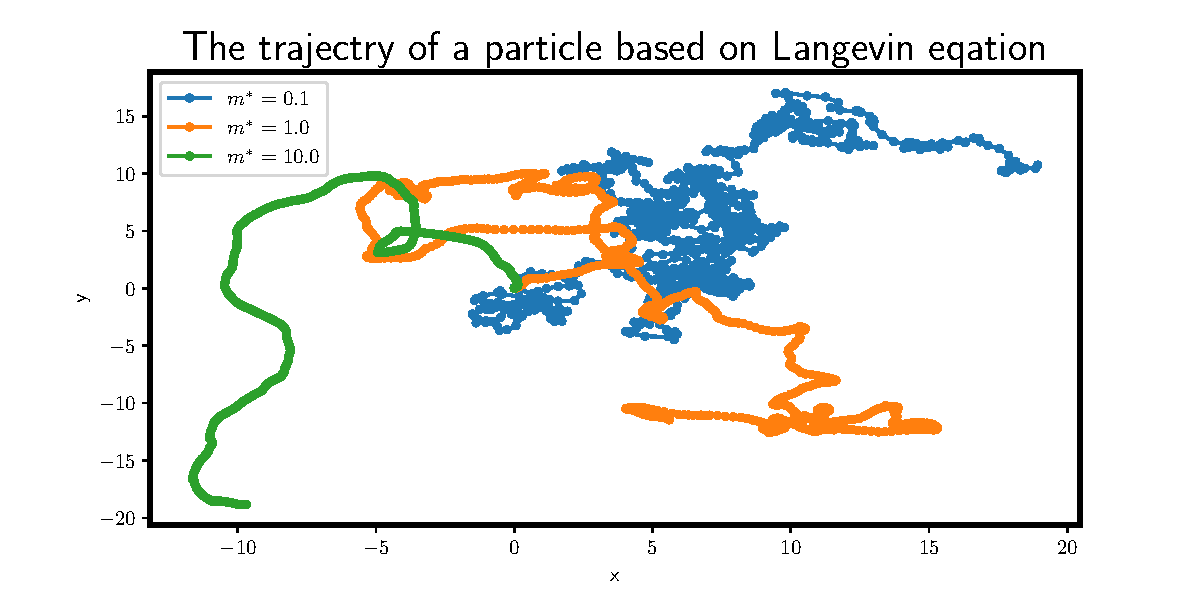
\includegraphics[scale=0.6]{problem_1/1-4/problem1-4.pdf}
    \caption{Langevin熱浴中における1粒子のブラウン運動}
\end{figure}
この図より, 慣性質量が大きくなるほど, 粒子軌道の範囲が狭まっていくことが分かる.


% (5)
\subsection{}
\noindent
(4)と同じ粒子について, 時間変化による平均二乗変位を


% 問題2
\section{}
% (1)
\subsection{}

\noindent

% \noindent
% 式(1)は定数係数の二階微分方程式より, $x=e^{\lambda x}$とおいて整理すると
% \begin{equation}
%     m\lambda^2 + \zzeta\lambda + k = 0 \tag{2.1}
% \end{equation}
% という特性方程式(2.1)を得る. この解は

% \begin{equation}
%     \lambda = \frac{-\zzeta + \sqrt{\zzeta^2 - 4mk}}{2} \tag{2.2}
% \end{equation}
% であり, ルートの中身について場合分けすると, 減衰振動, 過減衰, 臨界減衰を示す条件はそれぞれ

% \begin{align*}
%     \zzeta & > \sqrt{4mk}   (減衰振動) \tag{2.3}\\
%     \zzeta & < \sqrt{4mk}   (過減衰) \tag{2.4}\\
%     \zzeta & = \sqrt{4mk}   (臨界減衰) \tag{2.5}\\
% \end{align*}
% となる.


% \subsection{}

% \noindent
% 式(1)について$x = \tilde{x}$, $t = t_0 \tilde{t}$, $\dot{x} = v = \frac{a}{t_0} \tilde{v}$
% を代入して
% \begin{equation}
%     m \frac{a}{t_0} \dot{\tilde{v}}(\tilde{t}) = -\zzeta \frac{a}{t_0} \tilde{v}(\tilde{t})
%     -k a \tilde{x}(\tilde{t}) \tag{2.6}
% \end{equation}
% ここで

% \begin{align*}
%     \frac{d \tilde{v}(\tilde{t})}{dt} &= \frac{d \tilde{v}(\tilde{t})}{d \tilde{t}} \cdot \frac{d \tilde{t}}{dt} \\
%     &= \frac{1}{t_0} \frac{d \tilde{v}(\tilde{t})}{d \tilde{t}} \tag{2.7}
% \end{align*}
% より, 式(2.6)は

% \begin{equation}
%     \frac{m}{t_0^2} \frac{d \tilde{v}(\tilde{t})}{d \tilde{t}} = - \frac{\zzeta}{t_0} \tilde{v}(\tilde{t})
%     -k \tilde{x}(\tilde{t}) \tag{2.8}
% \end{equation}
% と表される. 式(2.8)左辺について, 刻み幅$\Delta \tilde{t}$に関するオイラー法による離散化を実行すると

% \begin{equation}
%     \frac{d \tilde{v}(\tilde{t})}{d \tilde{t}} = \frac{\tilde{v}(\tilde{t} + \Delta \tilde{t}) - \tilde{v}(\tilde{t})}{\Delta \tilde{t}} 
%     \tag {2.9}
% \end{equation}
% より, これを式(2.8)に代入して整理すると

% \begin{align}
%     \tilde{v}(\tilde{t} + \Delta \tilde{t}) = \left(1 - \frac{\zzeta t_0 \Delta \tilde{t}}{m}\right) \tilde{v}(\tilde{t})
%     - \frac{k t_0^2 \Delta \tilde{t}}{m} \tilde{x}(\tilde{t}) \tag{2.10}
% \end{align}
% また$\tilde{x}(\tilde{t} + \Delta \tilde{t})$について, 半陰的オイラー法に基づき

% \begin{align*}
%     \tilde{x}(\tilde{t} + \Delta \tilde{t}) &= \tilde{x}(\tilde{t}) + \tilde{v}(\tilde{t} + \Delta \tilde{t}) \Delta \tilde{t} \\
%     &= \left(1 - \frac{k t_0^2 \Delta \tilde{t}}{m}\right) \tilde{x}(\tilde{t}) 
%     + \left(1 - \frac{\zzeta t_0 \Delta \tilde{t}}{m}\right) \tilde{v}(\tilde{t}) \Delta \tilde{t} \tag{2.11}
% \end{align*}
% 以上より, 求める2項間漸化式は

% となる.

% % (3)
% \subsection{}

% \noindent
% 式(2.12)について$t_d = \frac{m}{\zzeta}$, $t_s = \sqrt{\frac{m}{k}}$を代入すると
% となる.

% % (4)
% \subsection{}
% \noindent

% 式(2.13)において$t_s=t_0$を代入し,さらに$\frac{t_0}{t_d}=T$とすると
% % \begin{subequations}
% %     \begin{align}
% %     \left\{
% %         \begin{aligned}
% %         & \tilde{v}(\tilde{t} + \Delta \tilde{t}) = \left(1 - T \Delta \tilde{t} \right) \tilde{v}(\tilde{t})
% %         - \tilde{x}(\tilde{t}) \Delta \tilde{t}\\
% %         & \tilde{x}(\tilde{t} + \Delta \tilde{t}) = (1 - \Delta \tilde{t} ) \tilde{x}(\tilde{t}) 
% %         + \left(1 - T \Delta \tilde{t} \right) \tilde{v}(\tilde{t}) \Delta \tilde{t}
% %         \end{aligned}
% %     \right} \tag{2.14}
% %     \end{align}
% % \end{subequations}
% となる.
% また, $t_d = \frac{m}{\zzeta}$, $t_s = \sqrt{\frac{m}{k}}$, $t_s=t_0$を式(2.3)-(2.5)に代入することで
% $\frac{t_0}{t_d}=T$とおいたとき
% \begin{align*}
%     T & < 2   (減衰振動) \tag{2.3}\\
%     T & > 2   (過減衰) \tag{2.4}\\
%     T & = 2   (臨界減衰) \tag{2.5}\\
% \end{align*}
% となるので, $T=0, 1, 2, 3, 4$のときの$x(t)$を図2.1にプロットした.
% 各$T$における$t$と$x(t)$の関係をproblem2.pyを用いて出力し, それらをproblem2.ipynb
% によって1つの図にプロットした. 
% ここで, $\Delta t=0.01$, $\frac{a}{t_0}=0.1$として計算し, $t$の範囲は(0,500)とした. 


\newpage
\noindent
※添付ファイル \\
・buffon.py \\
・ploblem2.py \\
・ploblem1.ipynb \\
・ploblem2.ipynb

\end{document}